
% THESIS CHAPTER

\chapter{Related work}
\label{chap:second}
\ifpdf
    \graphicspath{{Chapter2/Figures/PNG/}{Chapter2/Figures/PDF/}{Chapter2/Figures/}}
\else
    \graphicspath{{Chapter2/Figures/EPS/}{Chapter2/Figures/}}
\fi

% short summary of the chapter
\section*{Summary}
This chapter synthesizes the preliminary literature review explaining existing research, products end systems. It analyzes some robotics platforms and tools, in particular it presents an overview of existing autopilots boards and softwares. A suitable modeling technique for this kind of vehicles is described introducing additional non linearities and explaining when the model uses them.

Moreover it introduces a survey on various control techniques that are currently used highlighting pros an cons. \\*
At the end some comments are given about software architecture trends which are used in this field. 

\section{Quadrotor platform}

Flying objects have always exerted a great fascination on man encouraging all kinds of research and development. This intrigue for reaching the sky took all the form of imagination such as myths and legends. Many different and bizarre machines were theorized but very interesting were the precursors of the helicopter. Few visionaries, such as Leonardo da Vinci in the late 15th Century, foresaw an aerial application in the widely used windmill \cite{Heli} coming up with the famous screw design as propeller. Even if it never worked, Leonardo's design was very innovative and this challenge has generated centuries of frustration and hundreds of dramatic attempts without being fade. Only in 1933 Juan de la Cierva gave us the autogiro. The first pratical rotocraft invented which led to what we usually call helicopter. \par Few years after the first manned plane was invented, Dr. Cooper and Elmer Sperry designed the automatic gyroscopic stabilizer \cite{gyro}, which helps to keep an aircraft flying straight and level. This was the kick of unmanned vehicle research which has its starting point back to WWI and WWII. Few years later, sophisticated machines are seen in battle fields such as the famous Predator by General Atomics, the Hammeread by Piaggio Aerospace or the Pioneer by Israel Aerospace Industries. 
\begin{figure}[h]
\centering
 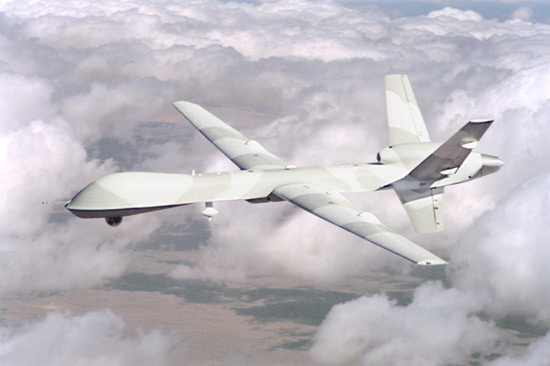
\includegraphics[width=0.7\textwidth]{predator.jpg}
 \caption[Predator UAV]{Predator Unmanned Aerial Vehicle }
 \label{figure:predator}
\end{figure}

\noindent
In the last ten years technology has taken a giant leap forward and the concept on Micro Aerial Vehicle (MAV) was born. Mavs are a class of UAVs with the feature of being relatively small and may be autonomous. Development is driven by commercial, research, government, and military purpose. The small craft allows remote observation of hazardous environments inaccessible to ground vehicles. MAVs have been built also for hobby purposes, such as aerial robotics contests and aerial photography.\par The union of Micro Aerial technology and the helicopter concept brings the quad rotor platform. Quadcopter, also known as quadrotor, is a helicopter with four rotors. The rotors are directed upwards and they are placed in a symmetric formation with equal distance from the center of mass. The quadcopter is controlled by adjusting the angular velocities of the rotors which are spun by electric motors.\par Designers came up with many projects and the market is now full of different vendors. The standard platform is the four propeller shape but
\begin{table}[h]
  \centering
  \begin{tabular}{ | c | m{5cm} | m{5cm} | }
    \hline
    Image & Description & Designer \\ \hline
   \parbox[c]{4cm}{
   \vspace{1ex}
      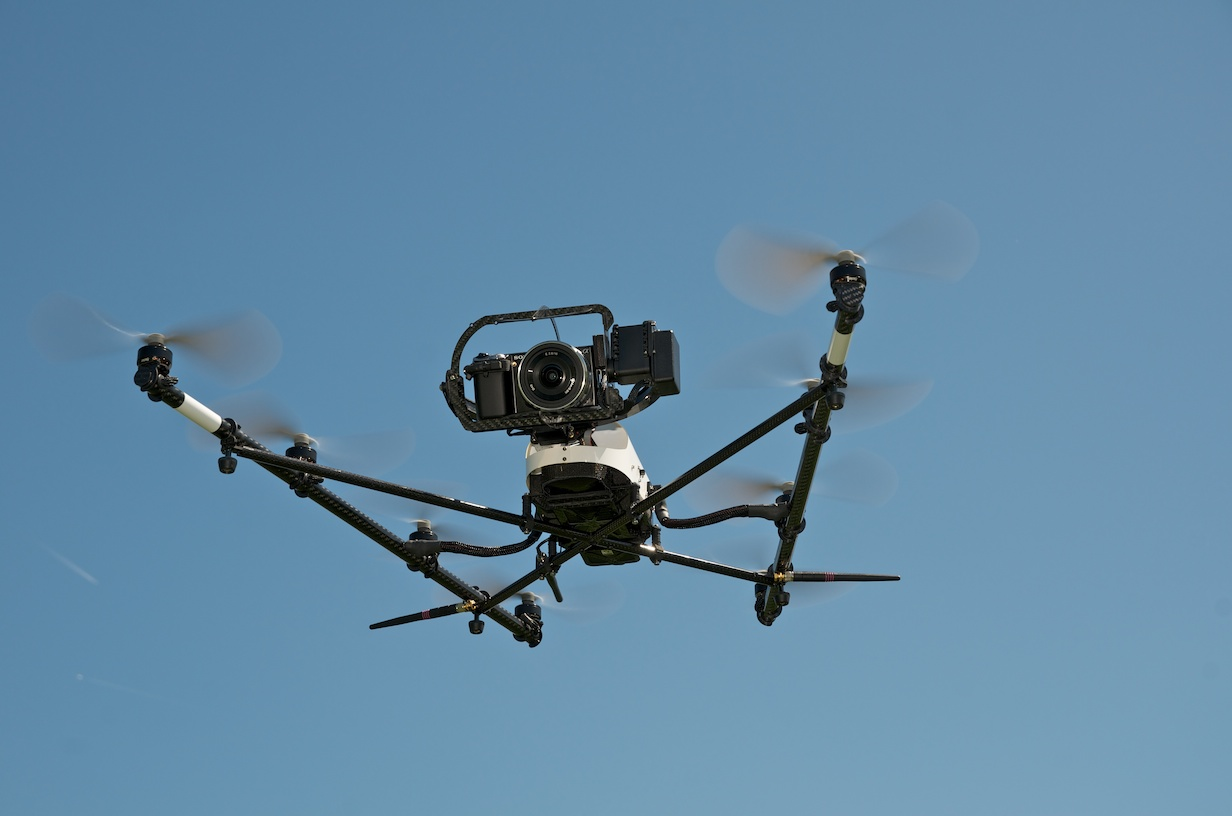
\includegraphics[width=\linewidth ]{Asctec_Falcon.jpg}
    }
    &
    \textbf{Falcon 8}, used by professionals for mapping and inspections.
    & 
   Produced by Ascending Technologies \cite{Ascend}
    \\ \hline
     \parbox[c]{4cm}{
      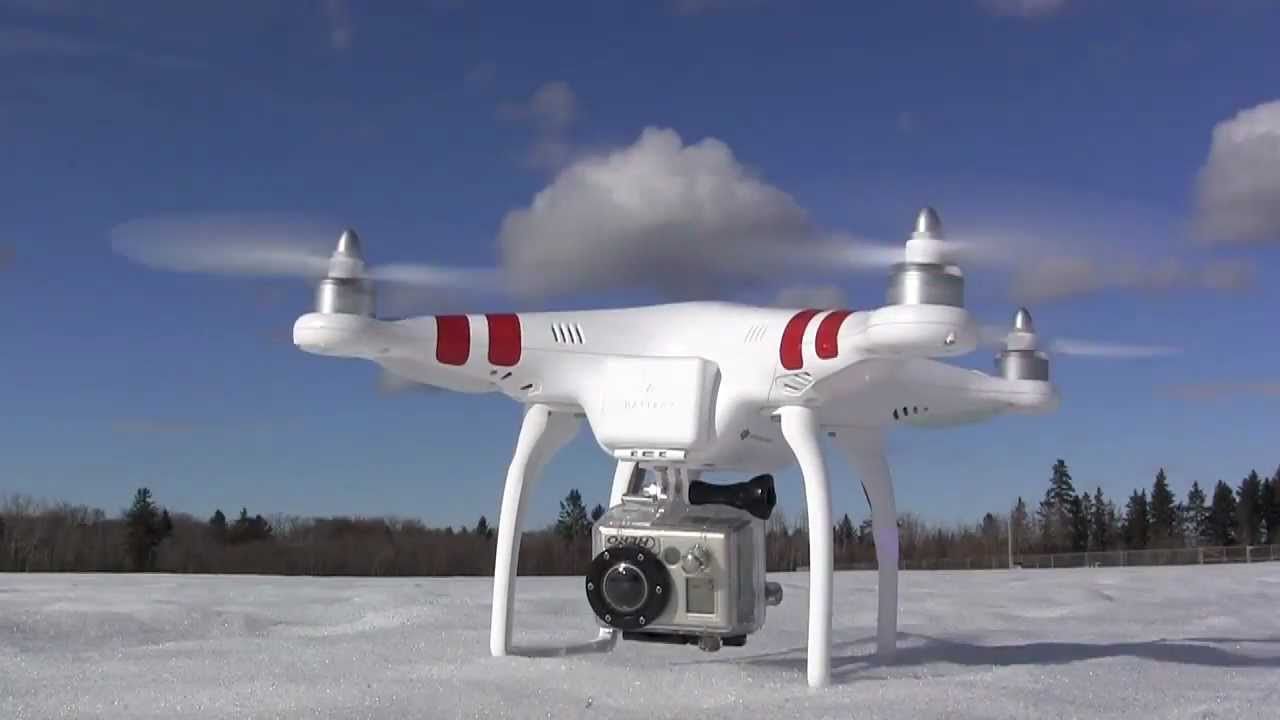
\includegraphics[width=\linewidth]{phantom.jpg}
   }
    & \textbf{Phantom 3}, ready to use high quality commercial platform.
    & Produced by DJI \cite{DJI}.
    \\ \hline
    \parbox[c]{4cm}{
      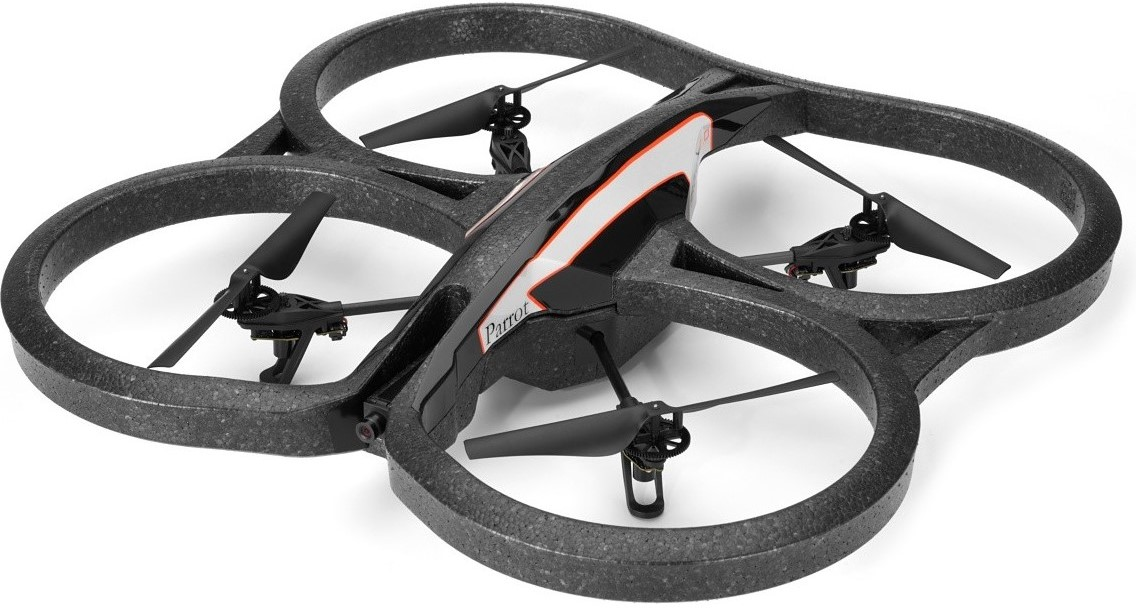
\includegraphics[width=\linewidth]{parrot.jpg}
   }
    & \textbf{AR.Drone}, ready to fly and cheap.
    & Produced by Parrot \cite{ARDrone}.
    \\ \hline 
     \parbox[c]{4cm}{
      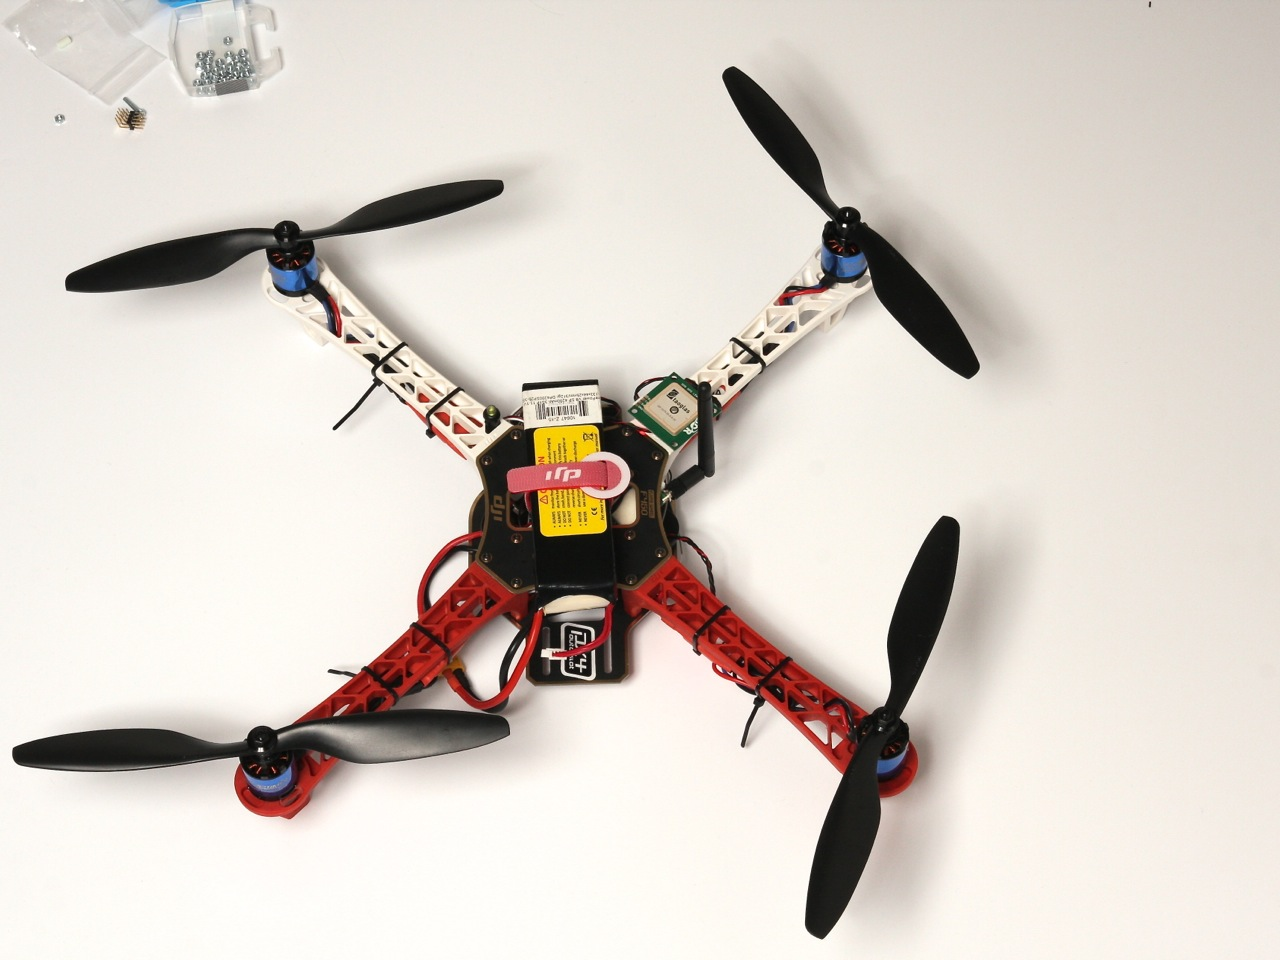
\includegraphics[width=\linewidth]{special_one.jpg}
   }
    & \textbf{Flamewheel}, this kit must be assembled by the user. Good quality.
    & Produced by DJI \cite{DJI} and assembled by Lorenz Meier \cite{Flamewheel} from PixHawk team.
    \\ \hline 
    \parbox[c]{4cm}{
      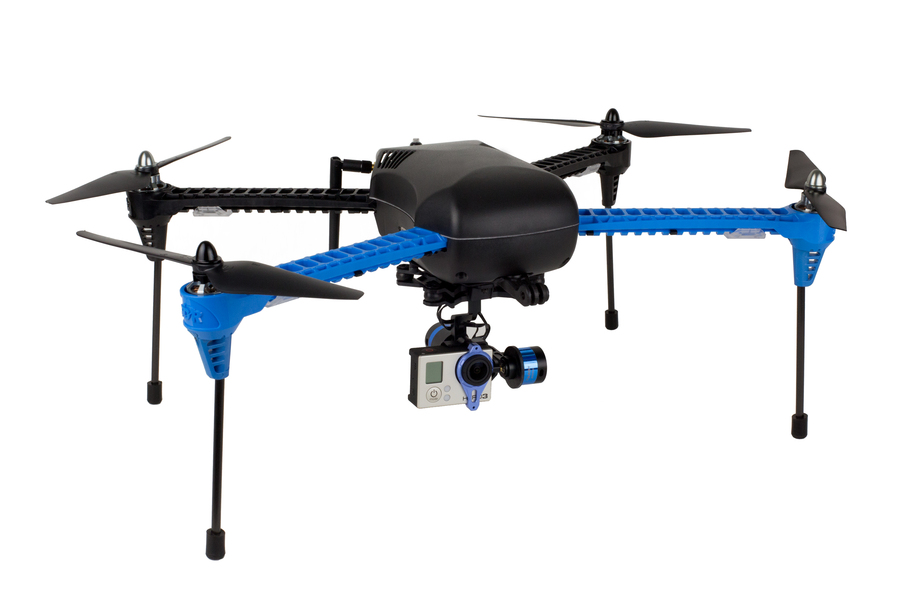
\includegraphics[width=\linewidth]{iri.jpg}
   }
    & \textbf{IRIS}, almost ready to use. High quality and robust but relatively cheap.
    & Produced by 3D Robotics \cite{3Dr}.
    \\ \hline 
    
      \end{tabular}
  \caption{Some copters designs}\label{tab:copters}
\end{table}
the architecture can be eventually expanded, with advantages and drawback, up to eight propellers. Those are eventually called octo-copters and they are made to transport heavy load but with very high power consumption. In order to choose the appropriate platform one must examine different models and evaluate which is the best based on the needs. We can divide copters available on the market in professionals, semi-professional, and not-professional.\par Professional copters are often used by qualified people in applications such as film making, inspection, mapping and surveillance. An example is the\textbf{ Falcon 8} by Asctec, it is very reliable and has fantastic performances. The price however is very high, it is not suitable to fly indoor and the autopilot is not open source. Some Asctec copters are designed for research but the price is too high for our purposes. Semi-professional copters are somewhat a step below the professional segment. Those copter are the most used among amateurs and they are very reliable. The \textbf{Phantom 3} is a well known platform, the quality is superb and it comes pre-assembled. Unfortunately the autopilot is not open source and an additional structure for IR markers must be added since the free surface is pretty tight. Another solution is to build from scratch the platform from a \textbf{Flamewheel} frame. In this case every piece is freely chosen, such as motors and autopilot, but the assembling process takes time and may lead to different issues. A very cheap solution is to use an \textbf{AR.Drone} by Parrot. It is absolutely ready to fly and the autopilot is not open source, even if it supports ROS integration. Thus we do not have the total control on the robot.
\par A quadrotor architecture is chosen for this thesis since they are more reliable, suitable for indoor application and more compact in  dimensions. IRIS from 3Dr (3D Robotics) is the experimental platform used in this project, it is almost ready to fly and very solid. The autopilot is open source and the price is relatively low. Table \ref{tab:copters} lists the platform illustrated in this section and a more detailed description of IRIS is given in \ref{sec:setup}.

\section{Motion capture systems}

Motion capture system, or mocap for short, is equipment specialized in the act of recording motion \cite{qualisys} usually through external sensors like cameras. Application of this technology are various and extended in different fields of science and not.\par In film making and media industry, mocap systems are used to track the motion of actors in order too translate it in a virtual environment for editing. This simplifies  the animation process and enable animators to capture the natural flow of human motion.\par Biomechanics is a very promising field and mocap systems plays an important role;  researchers and clinicians use motion data to study and observe human performance so they can improve treatment during rehabilitation as well as improve performance in sport applications. \par There are many industrial applications areas. From complex 3D vibration applications, vessel tracking above and under water, aerodynamics tests, automotive development, interior design and control design . The possibility to use motion capture underwater presents completely new possibilities to researchers in many application areas such as ship design, fishing industry and naval research.\par Mocaps are widely used in control systems where some feedback is necessary in order to generate some controlling signal. Robot performance analysis in particular is a field that widely uses mocap solutions.
\begin{figure}[h]
\centering
 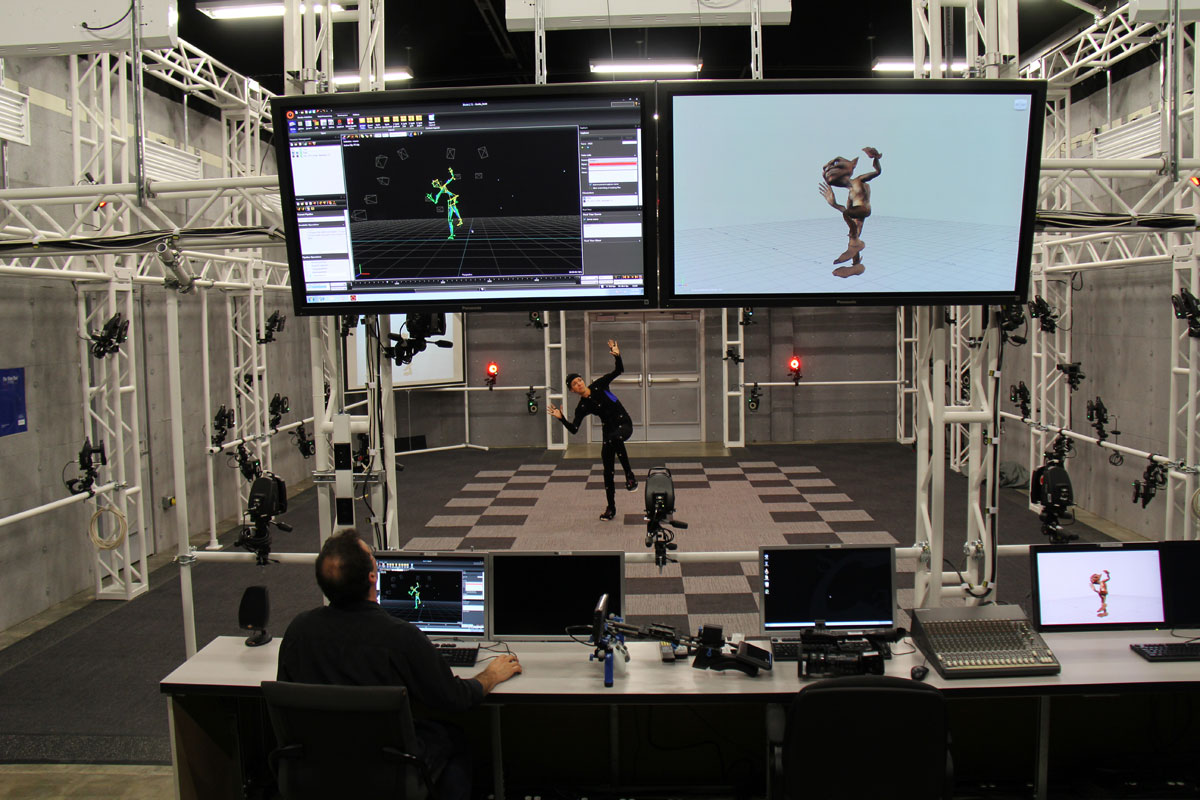
\includegraphics[width=0.7\textwidth]{motionstage.jpg}
 \caption[Motion capture stage]{An actor in a motion capture stage, the human movement is copied in a 3d model}
 \label{figure:motionstage}
\end{figure}

This technology is based on cameras able to detect Infra Red (IR) light. Every camera has a LED ring on it which fires IR beams, those beams are hence reflected by passive markers placed in advance on the object we want to observe. The reflected beams are finally detected by cameras and the software is able to reconstruct the position of each marker and the pose of the object.\par
There are different vendors for this kind of equipment but the most famous are OptiTrack \cite{OptiT} and Vicon \cite{vicon}. They both offer high-end technology and quality solutions, the choice is just matter of taste and which proprietary software is more suited.\par In the setup used in this project, the motion capture system consists in an OptiTrack Flex 13 with 8 cameras.


\section{Current autopilots}

The quadrotor architecture is a pretty old idea, it was not taken into account for long because people realized that in order to control four motors a decent amount of computing load and battery capacity are needed. However, the recent increase in electronic performances is why quadrotors are so famous right now.\par The actual trend is to pack every component in a small amount of space, this idea led producers to design \textbf{autopilot boards} with related software.

The most famous board is ArduPilot Mega \cite{ArduP}, a professional quality IMU autopilot that is based on the Arduino Mega platform.  This autopilot can control fixed-wing aircraft, multi-rotor helicopters, as well as traditional helicopters.  It is a full autopilot capable for autonomous stabilisation, way-point based navigation and two way telemetry with Xbee wireless modules. It is very simple to setup with their own utility hence no programming is required. The ArduPilot Firmware \cite{APM} is available on github and it is open source under GPLv3 licence. The 'Ardu' part in ArduPilot comes from the fact that originally this software was designed under Arduino environment. Eventually the project outgrown the Arduino platform and they become independent from Arduino run time libraries even if they are still supported. The community is huge, the documentation is very good and recently ArduPilot was used also in important rescue missions becoming the high end solution in commercial and DIY products.\par Till now APM seems to be the perfect choice from users stand point, but what about developers? Regarding this aspect some comments are necessary. When a new developer wants to contribute to a project the first thing he does is to check documentation and then experiment a bit with the code. From APM side, the documentation and support are superb \cite{APM}. The big drawback is the technical organization of the code. Since it started from Arduino platform but it evolved quickly, many changes where made. Some files kept the original Arduino extension '\textit{.pde}', some kept the famous \textit{.ino} while some other became part of a c library. There is a bit of confusion that could slow down the project, plus the code style is not very modern even if reliable.

On the other hand, IRIS features a PixHawk board (see \ref{sec:pixboard}) which by default supports APM but PX4 autopilot can be also installed. PX4\cite{PX4} is  described in \ref{sec:px4autop} and compared to APM has less features and less 'years of experience'. The community is still very active and the project it is growing very fast \cite{PX4Git}. It has every essential feature for an autopilot, just like APM it can be used on planes, helicopters, multicopters and rovers but the code is very organized an clear. The documentation is enough for a new developer , this why IRIS is running PX4 pilot in this project.

\section{Modeling and control}

The derivation of a dynamical model is the starting point for control design; quadrotor modeling was studied and explored extensively in the latest years with different complexity.\par Newton-Euler equations are widely used to handle quadrotor modeling as they lead to fairly simple results like in \cite{Michael2014}  and in \cite{Vendittelli}. A very common practice is to consider the robot as a rigid body, even if it it not true, and treat the aerodynamic propulsion separately. Since inputs of the system are the rates of each propeller, one can define some more realistic inputs calculating the relation of motors speed with force and torques generated \cite{Luukkonen2011}. Differential inputs are hence used. In \cite{Mahony2012} this principle is explained very well, the robot is described with rigid body equations where three torques and one force is applied. Propellers thrusts are calculated as proportional to the square of each rotor angular speed (\cite{Bouabdallah2007} and \cite{Mahony2012}). \par One may also consider some aerodynamic and additional non linear effects including them in the model and hence increasing accuracy. The simplest improvement could is to add friction with air as form of linear damping, called also drag. A more complex feature to model is called blade flapping \cite{Mahony2012}. In translational flight, the advancing blade of a rotor sees a higher effective velocity relative to the air, while the retreating blade sees a lower effective velocity. This results in a difference in lift between the two rotors, causing the rotor blades to flap up and down once per revolution \cite{Hoffmann2007} since they are pretty flexible. The last effect is that the total thrust varies not only with the power input, but also with the relative wind velocity.  \par Those effects are significant in aggressive maneuvering which include sudden change in direction and high speed hence they will not be taken into account. \\

\noindent
Controlling such system is a great challenge which arises many issues and proposal by scientific community, hence different controls have been applied to it. The quadrotor does not have complex mechanical control linkages due to the fact that it relies on variation in motor speed for vehicle control. However, these advantages come at a price. Controlling a quadrotor is not easy because of the coupled dynamics and its commonly under-actuated design configuration \cite{Algorithms2014}.
\par The most utilized controllers are: \begin{itemize}
\item PID control
\item Linear Quadratic Regulator
\item Feedback Linearization
\item Sliding Mode Control
\item Backstepping Control
\item Adaptive Control Algorithms
\end{itemize}
The \textbf{PID controller} has been applied to a broad range of applications. It is indeed the most use controller in industry. It is easily tuned even with empirical methods, it has good robustness and it is very easy to implement. It follows that PID it is applied also to quadrotors with fairly good results  especially in velocity control, attitude control and hovering \cite{Mahony2012}, \cite{Erginer2007}. However PID has some drawbacks due to the non linear nature of the system. Thus a linearization around hovering point is necessary \cite{Bouabdallah2} limiting quatrotor performances. Nevertheless PID is implemented most of commercial quadrotors available on the market. Hobbyists and developers mostly use PID for their platform because it is very simple to tune and it adapts to many structures and geometries. PX4 developers decided to adopt this kind of control in a cascaded fashion to improve adaptability respect to different quadrotor models. \par
\noindent
The \textbf{LQR optimal control} algorithm operates a dynamic system by minimizing a suitable cost function. Boubdallah and co-researchers applied the LQR algorithm to a quadrotor and compared its performance to that of the PID controller \cite{BouabdallahLQR}. LQR is in fact outperforming PID because it is designed on the full non linear system but still it does an average job. \par In the field of non linear control, the first technique is \textbf{Feedback Linearization}. It relies on putting a non linear system in a special form where it can be treated as linear. It was implemented on a quadrotor platform \cite{Altug2002} with good results. Nevertheless, feedback linearization presents an unforgivable drawback. The exact model must be know and this is never the case, in particular among DIY projects.\par \textbf{Sliding mode control} is another approach to non linear control. Sliding mode works by applying a discontinuous control signal to the system to command it to slide along a prescribed path thus achieving stability. The main advantages are the good tracking and  fact that there is no need to approximate the model dynamics. The discontinuous control signal may cause chattering and power loss. Sliding mode control is often used beside \textbf{backstepping} \cite{Bouadi2007} which is a recursive algorithm that breaks down the controller into steps and progressively stabilizes each subsystem. Its advantage is that the algorithm converges fast leading to less computational resources and it can handle disturbances well. The main limitation with the algorithm is its robustness is not good. \par More advanced tools are often used such as \textbf{Adaptive algorithms}. Adaptive control algorithms are aimed at adapting to parameter changes in the system. The parameters are either uncertain or varying with time and in many cases they were able to control systems where linearization failed. They were proven to be efficient in quadrotor control \cite{Antonelli2013} and the adaptive scheme could lead to many interesting results especially in presence of wind and during pick and place operations of small loads.\\ 

\noindent
To conclude this section I would like to point out one important aspect of PID control and why it is the selected algorithm for this project. There is a main difference between the presented algorithms: some are model dependent and some others are not. Feedback linearization for example is a very high model-dependent algorithm, same for dynamic canceling. It means that the perfect dynamical model must be known, the parameters well estimated and the dynamics well modeled. As experience teach, this is almost never the case. The PID is not model dependent, the choice of the gains makes it perfectly customizable for many structures and different type of rotor crafts. This is the key aspect on why it is mainly used, especially among amateurs.

\section{Software architectures and control stations}

A ground control station (GCS) usually is a land or sea-based control center that provides the facilities for human control of unmanned vehicles in the air or in space. A GCS could be used to control unmanned aerial vehicles or rockets within or above the atmosphere. It contains every feature needed to interact with the monitored system such as diagnostics, receive data and send commands, display vehicle state and perform emergency procedures. GCSs can be mobile or not and have different operational ranges. \par For aerial robotics usually the control station consists in a software running on a laptop or tablet and a communication module (radio, wi-fi , bluetooth). Let us have a brief look on which available solutions the market proposes and which is the choice for this project. \par 
Many companies offer proprietary solutions such as \textbf{Airware Control Station}  \cite{airware} but open source solutions are more reachable and expandable. ArduPilot supports \textbf{APM Planner} \cite{APMplan} which is the offspring of the well established and mostly used Mission Planner created by Michael Oborne. APM Planner is an open-source ground station application for MavLink(see \ref{sec:setup}) based autopilots including APM and PX4/Pixhawk that can be run on Windows, Mac OSX, and Linux. The most important features are: \begin{itemize}
\item Point-and-click waypoint entry, using Google Maps
\item Download mission log files and analyze them
\item Configure APM settings for user airframe
\item Interface with a PC flight simulator to create a full hardware-in-the-loop UAV simulator
\item Calibrate on board sensors
\item See vehicle status, parameters and sensors output

\end{itemize}
It is written using Qt libraries since they have good GUI support and is the first choice among hobbyists and professionals. It can be easily configured to  support different vehicles like boats, rovers, helicopters, multicopters and planes. \par APM Planner features are shared also by another popular GCS, especially among PX4 users, named \textbf{QGroundControl} \cite{QGround}. Additionally to APM PLanner, QGroundControl supports multiple vehicle instances at the same time which is essential in swarm robotics.  Moreover it has real time sensor plotting, in flight way points manipulation and digital video transmission from on board cameras. QGroundControl is used in this thesis to calibrate IRIS sensors and to tune some parameters. \par Those GCSs are cleary designed and optimized for outdoor missions, they have GPS support and displayed maps from Google Earth. Position feedback from another source such as a mocap system is not supported. What is lacking is a control station suitable for indoor application and experiments. During this work I designed a software architecture that takes the place of QGroundControl and it is aimed to be used with Optitrack cameras . The work of this thesis focuses more on the robot management than user experience and interface. It is written in Qt libraries because there could be a future integration with QGroundControl and because they offer many tools with a very good documentation. It sacrifices features such as Point-and-click waypoint entry and sensor calibration and it centralizes the robot performance and in particular robot autonomy. It is responsible of passing the robot position feedback from the mocap. The concept of task is presented as an action that IRIS can perform, the software scheduler takes a list of actions created by the user and let the robot execute them autonomously. This architecture is designed to be expanded as much as possible adding new tasks and modes.\par The main goal is to go towards a behavioral architecture for quadrotors, inspired by an old work by Montgomery James \cite{Montgomery1995}, and when the actions are sufficient integrate a planner to replace the user during the task list creation. Autonomy is the key aspect for this software, the idea is to abandon the figure of the mission operator and switch to a more autonomous system where the human role is just to set a goal.

\section{Landing on a moving platform}

Since many years people studied a way to land aircrafts safely, important studies has been made especially in the field of aerospace exploiting and designing different techniques to land spacecrafts on other planets. Moreover it happens that the target where the robot wants to land is not still, but performing some kind of motion on the ground. Landing a jet on an air carrier is a perfect example of a moving landing site, the platform is moving and possibly oscillating with waves.\par With the arrival of MAVs (Micro Aerial Vehicles) new challenges arise due to their dexterity and small sizes. Usually battery life is very limited and vehicles need to reach automatically recharge stations. A quadrotor may land on a moving car after its mission, on a robot in some cooperation task or on a floating boat to be recovered. All these procedures need a very high precision trajectory tracking and  perception of the environment.\\

\noindent
Small flying animals are capable of safe and accurate landings while relying only on proprioceptive sensors and visual information. Since this capability holds a promise of landing safely with limited sensors and processing, it has served as inspiration for recent spacecraft landing studies\cite{Izzo2012}. A very interesting research \cite{Baird2013} demonstrated how bees, with very simple measurements, are able to land on many surfaces. Dedicated eyes calculate the \textit{optical flow} of images meaning that they are able to track features and estimate the velocity of each feature in image plane. The results of this measurement is a vector field describing how a particular object (feature) in the image plane moves in time or from one frame to another in case of cameras. When one moves towards a surface with some pattern on, it is easy to experience an expansion towards the external edges of the image of the features (e.g. corners of a pattern). It is easy as well to feel this expansion faster as one is closer to the wall. Keeping this rate of expansion constant, bees are able to land easily. As closer they get to the surface, they measure a higher rate and in consequence they slow down to keep it constant. With this technique bees can safely land assuring that the approaching speed at touchdown is close to zero. \par
Another useful quantity that can be obtained from the optical flow is the Time To Contact, or TTC, defined also the ratio of the height and the vertical velocity. From this simple relation some descending control laws are derived \cite{Croon2015}. \\

\noindent
Those methods are developed assuming to have an optical flow sensor or a camera on board and pointing downwards. Unfortunately the IRIS does not have those features and we can rely only on the mocap and the IMU feedback. 
In this project the position of the platform will be estimated by the motion capture after putting markers on it, this may mimic a localized vehicle sending its position to the quadrotor ensuring the landing maneuver. \par The problem is separated in two different aspects, tracking and landing. In order to land tracking must be ensured and the research community proposed different methods. Some used non linear tracking \cite{Holger2008} and others, assuming that the velocity of the platform is estimated, compensate the delay of the robot respect to the target with a velocity feed-forward \cite{Friis2009}. A PI controller is synthesized in \cite{Herisse2010} closing a velocity control loop while a non linear control law assures the descending task. \par
Velocity control is not yet implemented in the software architecture and the only reference that is sent is a position set point. Hence I decided to rely only on position control, which may limit the performance of the maneuver but it is simple to implement and it is shown to be a valid strategy. \\
\noindent
The idea I followed is to remain as simple as possible avoiding non linear controllers. The experiment with bees, even if very interesting, do not take into account the tracking of a platform which must be integrated. Moreover it shows that bees use a linear law for descending: the vertical velocity decreases linearly with the height from the target. My algorithm is pretty simple but in some sense similar. The height of the IRIS decreases linearly with the horizontal position error respect to the center of the platform. This assures that the tracking has an higher priority respect to the landing, which will never occur if the robot is too far away. At the end tracking is made by a PI controller, closed respect the horizontal position error, with an offset. Since we hypothesized that velocity both for the robot and the platform is not available, feedback on position is the best way to solve the task. There are some drawbacks on using a PI controller such as the overshoot when the platform changes direction. Assuming that the motion of the landing site is smooth, the controller is able to secure the landing. 




























